\documentclass[12pt]{report}

\usepackage{listings}
\usepackage{xcolor}
\usepackage{graphicx}
\usepackage{amsmath}
\usepackage{hyperref}
\usepackage{geometry}
\usepackage{subfig}
\usepackage{float}
\usepackage{pgfplots}

\geometry{a4paper, margin=1in}
\pgfplotsset{compat=1.18}

\definecolor{codegray}{gray}{0.95}
\definecolor{codegreen}{rgb}{0.0, 0.5, 0.0}
\definecolor{codepurple}{rgb}{0.5, 0, 0.4}

\lstdefinestyle{cstyle}{
    language=C,
    backgroundcolor=\color{codegray},
    basicstyle=\ttfamily\footnotesize,
    keywordstyle=\color{codepurple}\bfseries,
    stringstyle=\color{orange},
    commentstyle=\color{codegreen},
    numbers=none,
    tabsize=4,
    showspaces=false,
    showstringspaces=false,
    frame=single,
    framerule=0.8pt,
    framesep=5pt,
    aboveskip=0.5cm,
    belowskip=0.5cm,
    breaklines=true,
}

\title{\textbf{Bitonic Sort with CUDA}}
\author{Ioannis Michalainas\\Maria Charisi}
\date{January 2025}

\begin{document}

\maketitle

\begin{abstract}
This report is part of an assignment for the \textbf{Parallel and Distributed Systems} class of the
Aristotle University's Electrical and Computer Engineering department, under professor \textit{Nikolaos Pitsianis}.

This project implements \textit{parallel sorting} using the \textbf{Bitonic Sort} algorithm and the \textbf{CUDA} framework. The primary objective is to sort a dataset of $N = 2^k$ numbers (where $k \in \mathbb{N}$). The implementation employs parallel processing to achieve efficient sorting, making it suitable for large-scale data sets.
\end{abstract}

\tableofcontents

\vfill
\begin{center}
    \textit{Professor: Nikolaos Pitsianis\\
    Department of Electrical and Computer Engineering\\
    Parallel and Distributed Systems}
\end{center}
\newpage

\chapter{Serial Bitonic}

To grasp the concept of distributed \textbf{Bitonic Sort}, it is essential to first understand its serial implementation. This foundational knowledge will provide the necessary context for comprehending the distributed version of the algorithm.

\section{Explanation}

\textbf{Bitonic Sort} is a sorting algorithm that operates by sorting and merging bitonic sequences. A bitonic sequence is defined as a sequence of numbers that first monotonically increases and then monotonically decreases (or vise versa), or can be cyclically rotated to exhibit this pattern. Note that sorted sequences are also bitonic. For example, the sequence $6, 4, 3, 1, 2, 5, 8, 7$ is bitonic because it can be rotated to $7, 6, 4, 3, 1, 2, 5, 8$. 

The algorithm has the following characteristics:
\begin{itemize}
    \item $log(n)$ steps, where n is the total amount of numbers, with $step$ comparison phases in each step.
    \item In each comparison phase, we swap elements using the \textbf{min-max} criteria. The Min-Max pattern is presented in the image below:
\end{itemize}

\begin{figure}
    \centering
    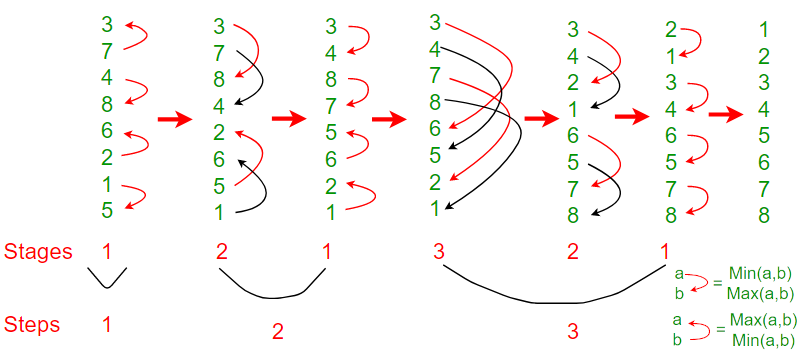
\includegraphics[width=0.9\linewidth]{assets/bitonic.png}
    \caption{Bitonic Sort}
    \label{fig:enter-label}
\end{figure}
\section{Example}

To illustrate the process, consider the following random sequence:
\[S\{ 3,7,4,8,6,2,1,5 \}\]
In each step each element is compared to its neighbor with distance \textbf{stage}.

\begin{enumerate}
    \item \textbf{Step 1, Stage 1}
    \textbf{min-max pattern:} $min\:max\:max\:min\:min\:max\:max\:min$
    \[
        S\{3,7,8,4,2,6,5,1\}
    \] 
    \item \textbf{Step 2, Stage 2}
    \textbf{min-max pattern:} $min\:min\:max\:max\:max\:max\:min\:min$
    \[
        S\{3,4,8,7,5,6,2,1\}
    \]
    \item \textbf{Step 2, Stage 1}
    \textbf{min-max pattern:} $min\:max\:min\:max\:max\:min\:max\:min$
    \[
        S\{3,4,8,7,6,5,2,1\}
    \]
    \item \textbf{Step 3, Stage 3}
    \textbf{min-max pattern:} $min\:min\:min\:min\:max\:max\:max\:max$
    \[
        S\{3,4,2,1,6,5,7,8\}
    \]
    \item \textbf{Step 3, Stage 2}
    \textbf{min-max pattern:} $min\:min\:max\:max\:min\:min\:max\:max$
    \[
        S\{2,1,3,4,6,5,7,8\}
    \]
    \item \textbf{Step 3, Stage 1}
    \textbf{min-max pattern:} $min\:max\:min\:max\:min\:max\:min\:max$
    \[
        S\{1, 2, 3, 4, 5, 6, 7, 8\}
    \]
\end{enumerate}

\section{Remarks}

\begin{enumerate}
\item The complexity of this algorithm is $O(nlog^2n)$. While it is higher than other popular sorting algorithms like \textbf{Merge Sort} or \textbf{Quick Sort},  \textbf{Bitonic Sort} is ideal for parallel implementation, because it always compares elements in a predefined sequence and the sequence of comparison does not depend on data. 
\item \textbf{Bitonic Sort} can only be used if the number of elements to sort is $2^n$. The procedure fails if the number of elements is not in the aforementioned quantity precisely.
\end{enumerate}
        
\chapter{Parallel Bitonic}
As mentioned above, this algorithm, when implemented in a serial manner, has a time complexity of \(\boldsymbol{O(n\log^2(n))}\), which is higher than most sorting algorithms. Despite that, this algorithm is useful, as it is well-suited for parallel implementations. With parallelism, it has a time complexity of \(\boldsymbol{O(\log^2(n))}\), which is significantly faster than our serial implementation. We will be achieving this goal with \textbf{CUDA}, allowing us to distribute the load across multiple threads on a GPU.

\section{V0}
Similarly with the serial algorithm, in order to sort a sequence we go through $\log(N)$ stages and in each stage $\log(stage)$ exchanges happen. 
\begin{lstlisting}[style=cstyle]
for (int stage=2; stage<=n; stage<<=1) {
    for (int step=stage>>1; step>0; step>>=1) {
        bitonicExchange<<<blocks, THREADS_PER_BLOCK>>>(d_arr, threads, stage, step);
        cudaDeviceSynchronize();
    }
}
\end{lstlisting}

\subsection{Exchange}

Each thread \textbf{exchanges} data with its \textbf{partner}. We need to determine the \textbf{distance} of the partner that the thread should exchange data with, in our case $step$. We then calculate the partner based on the distance: $$tid \:\: XOR \:\: step$$

The threads are arranged in a hypercube-like structure, where the global id of each thread is treated as a binary number. The \textbf{XOR} operation between two binary numbers results in a number where the bits are set to 1 at positions where the two numbers differ. The distance between two nodes in a hypercube is the number of differing bits between their binary representations, known as the \textbf{Hamming distance}. 

\begin{figure}[H]
    \centering
    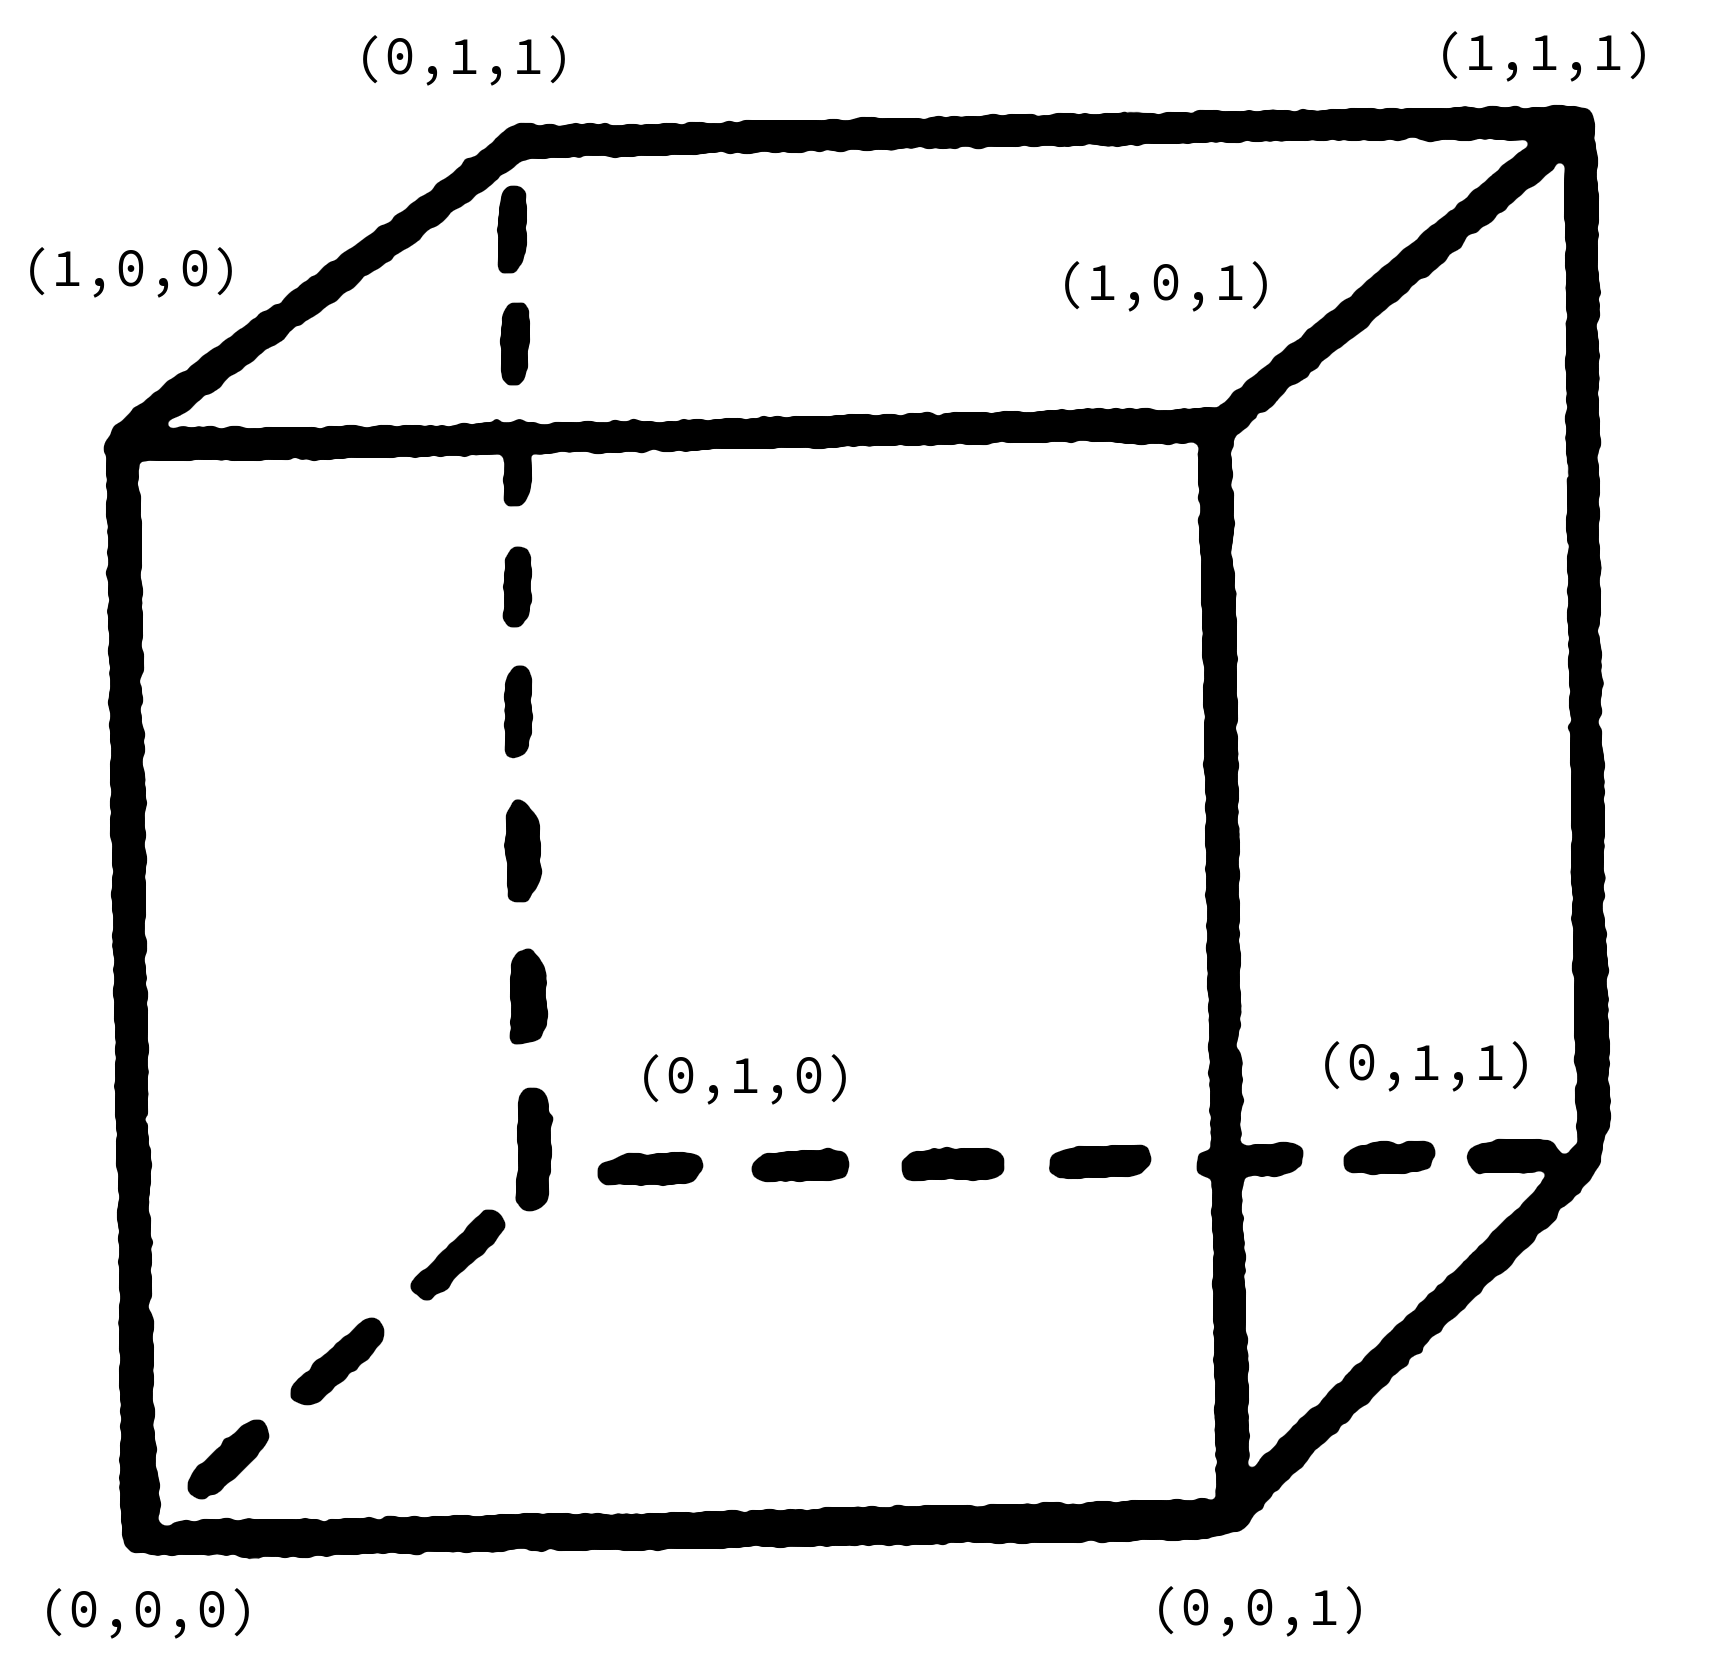
\includegraphics[width=0.5\linewidth]{assets/cube.png}
    \caption{3D Hyper-Cube Representation}
    \label{fig:enter-label}
\end{figure}

The XOR operation helps find a partner that differs from the current thread by exactly the number of bits defined by the \textit{distance} at each step. This ensures that in each stage of the algorithm, the thread exchanges with a partner that is located at a specific Hamming distance, consistent with the hypercube structure. At each stage, the \textit{distance} doubles (based on the step), and the \verb|tid ^ distance| operation calculates a thread ID that is at the desired Hamming distance.

\subsection{Compare}

Once each thread has identified a partner, we need to establish the min-max criteria to determine which partner retains the highest number and which the lowest.

\begin{lstlisting}[style=cstyle]
bool minmax = (tid & stage) == 0;
\end{lstlisting}

The above condition accurately reflects the min max pattern we need to follow in each stage to end up with a sorted array.

\subsection{Number of Threads}

In CUDA, the number of threads available per block is fixed and equal to $2^10$ (1024). To calculate how many blocks we need to have the required threads to perform our operations we use the following formula. 

\begin{lstlisting}[style=cstyle]
int blocks = (threads-1) / THREADS_PER_BLOCK+1;
\end{lstlisting}

For our parallel implementation, we assign one GPU thread for every two numbers. Meaning, if we have $N$ numbers to sort, we employ $N/2$ threads, each one responsible for comparing and exchanging (if needed) its partner numbers. That way, we have 50\% more threads for further calculations. Using a GPU with $2^N$ total threads, we can sort an array with $2^{N+1}$ elements. 

\begin{lstlisting}[style=cstyle]
__global__ void bitonicExchange(int* arr, int threads, int stage, int step) {

    unsigned int tid = threadIdx.x + blockDim.x*blockIdx.x;
    if (tid < threads) {

        unsigned int partner = tid^step;
        if (partner > tid) {
            bool minmax = (tid & stage) == 0;
            swap(arr, tid, partner, minmax ? arr[tid] > arr[partner] : arr[tid] < arr[partner]);
        } else {
            tid += threads;
            partner += threads;

            bool minmax = (tid & stage) == 0;
            swap(arr, tid, partner, minmax ? arr[tid] < arr[partner] : arr[tid] > arr[partner]);
        }
    }
}
\end{lstlisting}

It is possible to have a block with extra threads that do not correspond to any part of the array. To remedy that, we discard any excess threads evoked beyond $N/2$. The lower partner tid handles the exchange on the first half of the array while the higher partner gets shifted by half the array size to handle exchanges on the later half. That way, when two threads partner with each other both of them perform calculations and none remains idle.

\subsection{Synchronization}

There is a glaring downside to the V0 implementation. While easy to write, V0 requires multiple kernel calls. We need to call cudaDeviceSynchronize() order of $log(n)^2$ times to avoid race conditions. Global synchronizations are generally slow, taking a toll on our implementation. \newpage

\section{V1}

In V1 we improve on V0 by attempting to reduce the function calls and global synchronizations. The idea is to include the step loop in the kernel, replacing global synchronizations with block syncs. However, for numbers bigger that $2^{10}$ (1024) we exceed the threads per block limit of CUDA. In these cases we employ the previous V0 logic.

\begin{lstlisting}[style=cstyle]
localSort<<<blocks, THREADS_PER_BLOCK>>>(d_arr, n, 1<<1, 1<<0);
for (int stage=1<<11; stage<=n; stage<<=1) {
    for (int step=stage>>1; step>1<<9; step>>=1) {
        bitonicExchange<<<blocks, THREADS_PER_BLOCK>>>(d_arr, threads, stage, step);
        cudaDeviceSynchronize();
    }
    localSort<<<blocks, THREADS_PER_BLOCK>>>(d_arr, n, stage, 1<<9);
}
\end{lstlisting}

To do this, we need two kernels, one handling stages bigger than $2^{10}$, the previous bitonicExchange kernel and the other performing calculations faster for [stages, steps] up to [1024, 512]. The second kernel is faster, because every block of threads works on a distinct part of the array. No synchronization with the other blocks is required, allowing each block to work in its own rhythm.

\begin{lstlisting}[style=cstyle]
__global__ void localSort(int* arr, int n, int stage, int step) {

    unsigned int tid = threadIdx.x + blockDim.x*blockIdx.x;
    unsigned int offset = n>>1;
    if (tid < (n>>1)) {
        do {
            while (step>0) {
                
                unsigned int partner = tid^step;
                if(partner > tid){
                    bool minmax = (tid & stage) == 0;
                    swap(arr, tid, partner, minmax ? arr[tid] > arr[partner] : arr[tid] < arr[partner]);
                } else {
                    tid += offset;
                    partner += offset;

                    bool minmax = (tid & stage) == 0;
                    swap(arr, tid, partner, minmax ? arr[tid] < arr[partner] : arr[tid] > arr[partner]);

                    tid -= offset;
                }
                step >>= 1;
                __syncthreads();
            }
            stage <<= 1;
            step = stage >> 1;
        } while (stage <= min(n, 1<<10));
    }
}
\end{lstlisting}

\section{V2}

V2 is essentially another improvement on V1. Instead of using global memory in the localSort kernel, we use shared memory within each block, in an attempt to speed up the process.

\begin{lstlisting}[style=cstyle]
__global__ void localSort(int* arr, int n, int stage, int step) {

    extern __shared__ int sharedArr[];
    unsigned int globalId = threadIdx.x + blockDim.x*blockIdx.x;
    unsigned int localId = threadIdx.x;
    unsigned int offset = min(n>>1, blockDim.x);

    if (globalId < (n>>1)) {
        
        sharedArr[localId] = arr[globalId];
        sharedArr[localId + offset] = arr[globalId + (n>>1)];
        __syncthreads(); 

        ...

        arr[globalId] = sharedArr[localId];
        arr[globalId + (n>>1)] = sharedArr[localId + offset];
        __syncthreads();
    }
}
\end{lstlisting}

Each block of threads is tasked with comparing and exchanging elements in two sections of the array: one corresponding to its native location and the other determined by the shifted thread IDs. To facilitate this process, we require a shared memory array of size 2*THREADS\_PER\_BLOCK*sizeof(int) (2048) for each block. When the kernel is executed, the relevant portions of the array are loaded from global memory into the block's shared memory. After completing the operations, the results are written back to global memory.

\chapter{Results}
As previously mentioned, a serial version of this algorithm has a time complexity of $\boldsymbol{O(n \log^2(n)}$, which is not ideal, as there are faster algorithms. However, a parallel version, significantly lessens this to $\boldsymbol{O(\log^2(n))}$.

\begin{table}[h!]
    \centering
    \begin{tabular}{|c|c|c|c|}
        \hline
        \rule{0pt}{3ex}\textbf{Performance Table} & \textbf{Serial}                 & \textbf{Parallel}          & \textbf{Quick Sort}          \\ \hline
        \rule{0pt}{3ex}Time Complexity            & \(\boldsymbol{O(n \log^2(n))}\) & \(\boldsymbol{O(\log^2(n))}\) & \(\boldsymbol{O(n\log(n))}\) \\ \hline
    \end{tabular}
    \caption{Performance Table}
    \label{tab:simple_table}
\end{table}

\begin{center}
    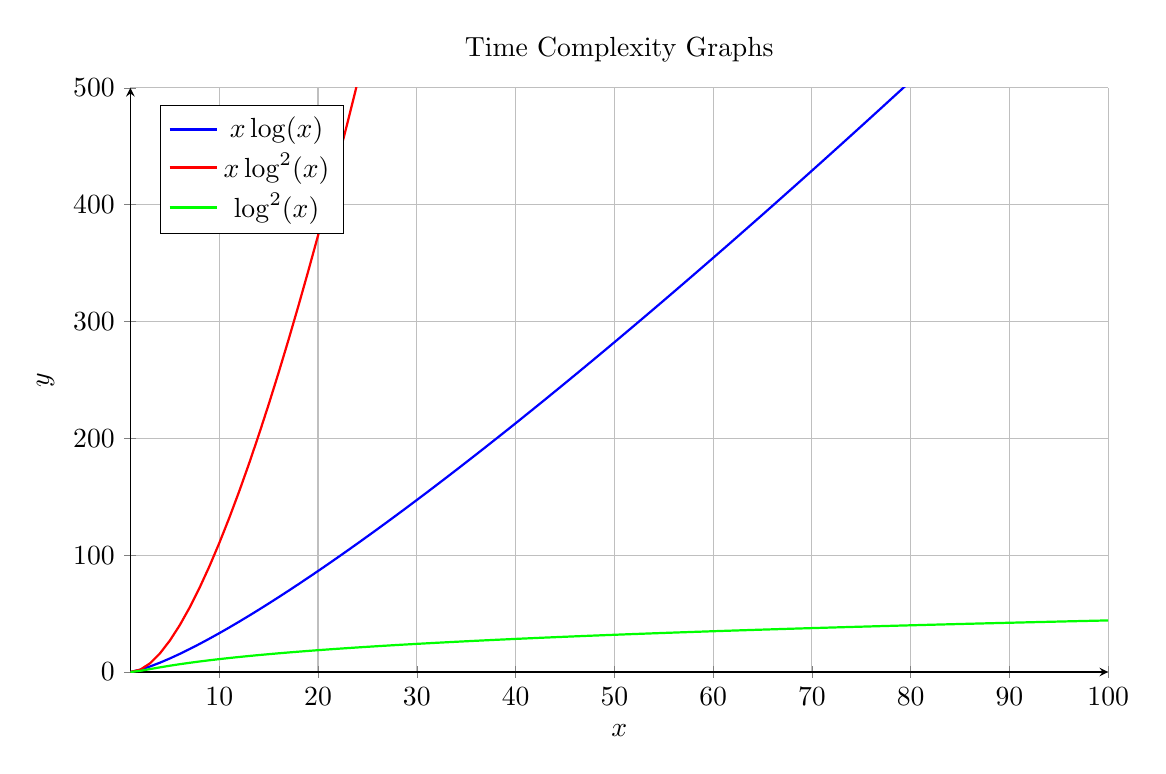
\begin{tikzpicture}
        \begin{axis}[
            width=14cm,
            height=9cm,
            xlabel={$x$},
            ylabel={$y$},
            xmin=1, xmax=100,
            ymin=0, ymax=500,
            legend pos=north west,
            grid=major,
            axis x line=bottom,
            axis y line=left,
            title={Time Complexity Graphs}
        ]
            % plot x*log2(x)
            \addplot[blue, thick] expression[domain=1:100, samples=100]{x * ln(x)/ln(2)};
            \addlegendentry{$x \log(x)$}

            % plot x*(log2(x))^2
            \addplot[red, thick] expression[domain=1:100, samples=100]{x * (ln(x)/ln(2))^2};
            \addlegendentry{$x \log^2(x)$}

            % plot (log2(x))^2
            \addplot[green, thick] expression[domain=1:100, samples=100]{(ln(x)/ln(2))^2};
            \addlegendentry{$\log^2(x)$}
        \end{axis}
    \end{tikzpicture}
\end{center}

This program was executed on a Windows machine with a \textbf{NVIDIA GeForce GTX 750} GPU. We used CUDA 11.8 to accommodate the low compute capability (5) of the specific graphics card. We tested for values of N in the range [16..27], where the total numbers are $2^N$. \newpage

In the graphic below, we observe the \textit{performance} of the algorithm for different values of $n$, compared to qsort. 

\begin{figure}[H]
    \centering
    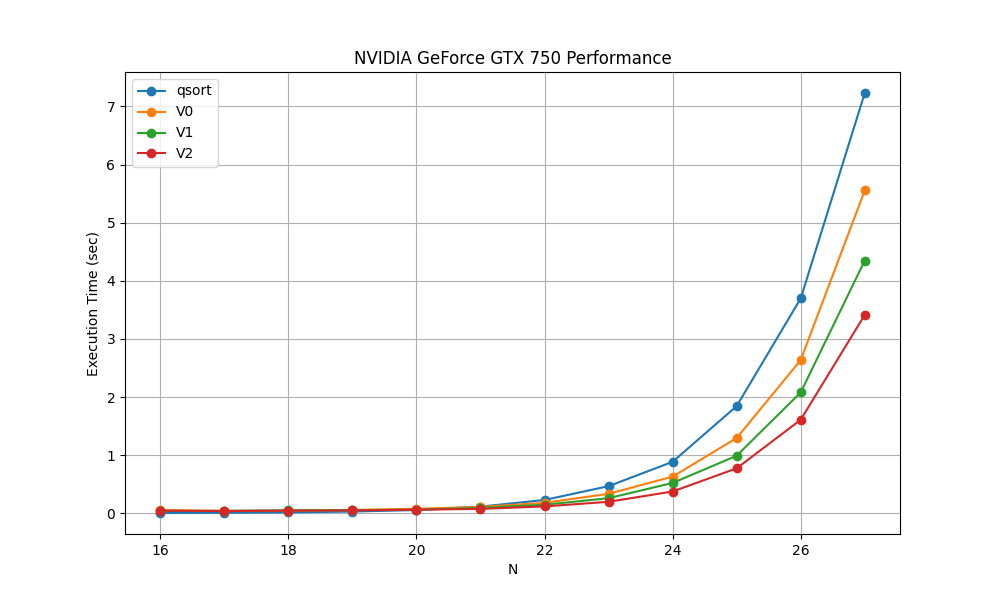
\includegraphics[width=1\linewidth]{assets/GTX750.png}
    \caption{Performance}
    \label{fig:enter-label}
\end{figure}

\chapter{Tools and Sources}

In this project, the following tools where used:
\begin{enumerate}
    \item The \textbf{C} programming language.
    \item The \textbf{CUDA} framework for implementing the parallel algorithm.
    \item The \textbf{Aristotle Cluster} for testing.
    \item \textbf{VSCode} IDE for development.
    \item \textbf{GitHub} for version control.
    \item \textbf{GitHub Copilot} as an AI assistant.
    \item \textbf{Python} with \textbf{matplotlib} for graphics
    \item \textbf{Gimp} for asset creation.
\end{enumerate}

The following sources were helpful for understanding the problem presented in the assignment:
\begin{itemize}
    \item \url{https://www.geeksforgeeks.org/bitonic-sort/}
    \item Lecture notes from the \textbf{Parallel and Distributed Systems} course, written by professor \textbf{Nikolaos Pitsianis}.
\end{itemize}

\end{document}